\section{Esempi Esecuzione}
Di seguito illustreremo il funzionamento  di alcune funzioni introdotte all'interno della sezione \ref{funzioni}
\subsection{Docente}
prendiamo la tabella docente (\ref{tab:docente})

fatto questo procediamo a testare la funzione \ref{checkdocentetr} \textit{check\_docente\_tr}, provando a lanciare la linea: 
\begin{lstlisting}[style=sqlStyle]
INSERT INTO "docente" ("email", "pass", "nome", "cognome")
VALUES ('docente@example.com', 'password', 'mario', 'rossi');

\end{lstlisting}

\begin{figure}[ht]
    \centering
    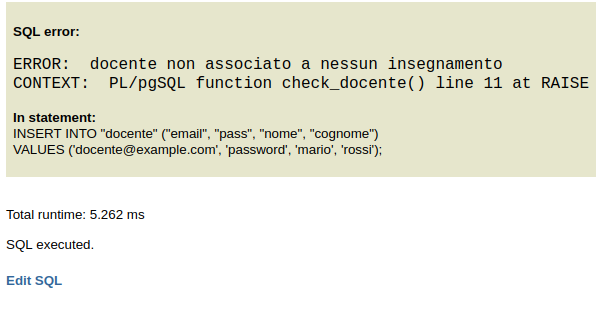
\includegraphics[width=0.9\linewidth]{images/createDocente.png}
    \label{error:createDoncenteInsert}
\end{figure}
come possiamo vedere in figura \ref{error:createDoncenteInsert} l'inserimento  non è andato a buon fine in quanto il trigger è scattato e ha impedito l'inserimento.


Se invece lanciassimo  la seguente linea dove creiamo un docente e gli associamo un insegnamento il cui id è 1 (dando pe assunto che l'insegnamento sia già presente nella tabella \textit{insegnamento}

\begin{lstlisting}[style=sqlStyle]
select * from create_docente('docen00te@example.com', 'password', 'mario', 
'rossi','2010-05-01',1);
\end{lstlisting}
otteremo il seguente risultato 
\begin{figure}[ht]
    \centering
    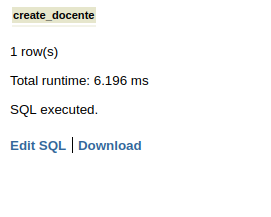
\includegraphics[width=0.2\linewidth]{images/succcesCrateDocente.png}
    \label{succ:creaDocenmtefc}
\end{figure}
notiamo come in questo caso tutto proceda correttamente e che il docente venga creato correttamente l'insegnamento riceva il proprio responabile,prima null, associato.

E se cercassimo di associare un docente ad un insegnamento con già un responsabile? 
\begin{figure}[ht]
    \centering
    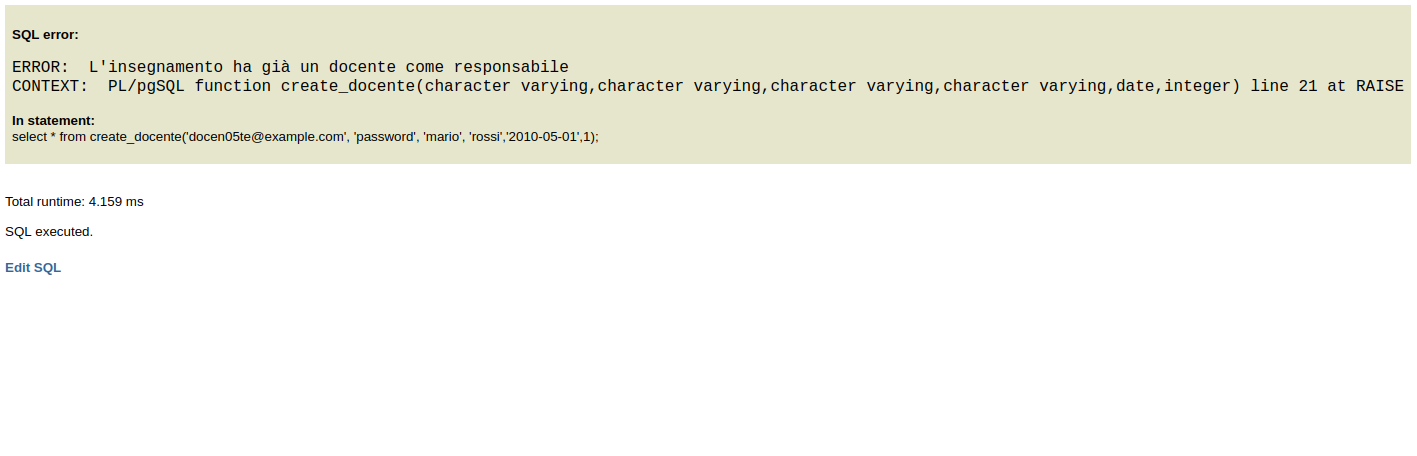
\includegraphics[width=0.9\linewidth]{images/createDocenteResponsabileError.png}
    \label{succ:creaDocenmteErrorResp}
\end{figure}

Restando in tema della colonna responsabile è doveroso notare come se si decidesse di associare più di 3 insegnamenti ad un docente  il trigger \textit{docente\_insegnamento\_tr} riportado l'errore  \textit{'Limite massimo raggiunto'}
\subsection{Carriera}
il funzionamemto delle funzioni carriera sono identiche tra loro, cambia soltanto con che criterio sono presi i voti,per questo motivo ne mostreremo soltanto uno:
\begin{lstlisting}[style=sqlStyle]
 SELECT * FROM get_carriera_valida('123456');
\end{lstlisting}
\begin{figure}[ht]
    \centering
    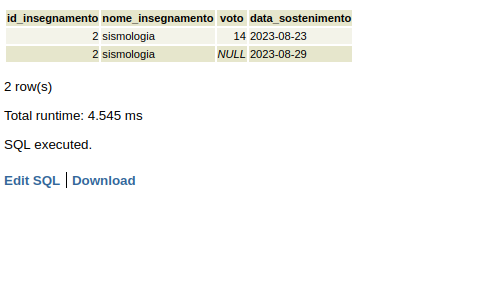
\includegraphics[width=0.9\linewidth]{images/getCarriera.png}
    \label{succ:creaDocenmteErrorResp}
\end{figure}

\subsection{Appello}
Per la creazione di un appelle ogni volta che viene eseguito controlla che non sia in conflitto con il trigger
\begin{lstlisting}[style=sqlStyle]
INSERT INTO appello VALUES ('2023-04-30','aula 200'1);
INSERT INTO appello VALUES ('2023-04-30','aula 202,2);
\end{lstlisting}
queste linee presuppongono chiaramente la presenza di due insegnamenti appartenenti allo stesso corso di laurea e con lo stesso anno consigliato 
\begin{figure}[ht]
    \centering
    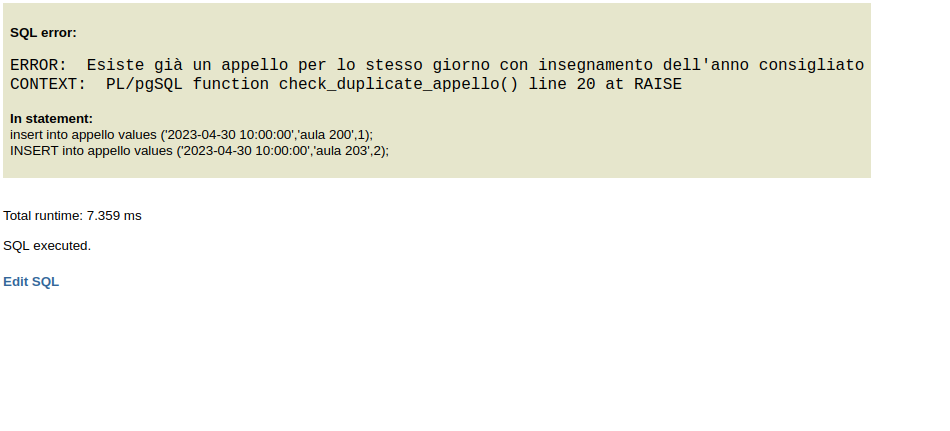
\includegraphics[width=0.9\linewidth]{images/sovrapposizione.png}
    \label{err:sovrapposizioneAppello}
\end{figure}
\subsection{CFU}
per la gestione dei voti e dei cfu utilizziamo la funzione \textit{add\_voto} la quale peremette,se uno studente è iscritto ad un esame, di assegnare un voto nella tabella appello la quale poi prosegue aggiornando i cfu in caso di voto superiore al 18.

Ipotiziamo di avere un insegnamento con id=1 e un numero di cfu pari a 6 e di avere un appello a cui lo studente è iscritto per il 2023-08-17 10:00:00. 

Questo saranno gli studenti, ci concentreremo su quello con matricola="mam":
\begin{figure}[ht]
    \centering
    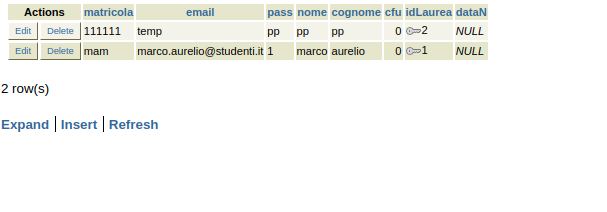
\includegraphics[width=0.9\linewidth]{images/studenti1.png}
\end{figure}
lanciando quindi la seguente  linea:
\begin{lstlisting}[style=sqlStyle]
SELECT add_voto(30, 'mam', 1, '2023-08-17 10:00:00');
\end{lstlisting}
questa linea assegnarà il voto 30 all'appello e il risulterà nella modifica dei cfu
\begin{figure}[ht]
    \centering
    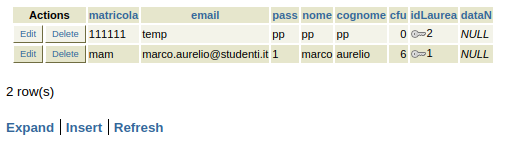
\includegraphics[width=0.9\linewidth]{images/studenti2.png}
\end{figure}